% Standalone figure for ICTer 2026 submission.
% Compile this file separately to produce fig1.pdf, then include it in weave.tex.
% The figure is also embedded directly in weave.tex as inline TikZ,
% so this file is only needed if the conference requires a separate figure file.
%
% Compile: pdflatex fig1.tex
\documentclass[border=5pt]{standalone}
\usepackage[T1]{fontenc}
\usepackage{times}
\usepackage{tikz}
\usepackage{amsmath}
\usetikzlibrary{positioning,arrows.meta,fit,calc}

\definecolor{cwmblue}{HTML}{2E5E8C}
\definecolor{oursorange}{HTML}{C8552B}
\definecolor{barfill}{HTML}{C8552B}
\definecolor{panelgray}{HTML}{F2F2F2}
\definecolor{panelborder}{HTML}{BBBBBB}
\definecolor{labelone}{HTML}{555555}

\begin{document}
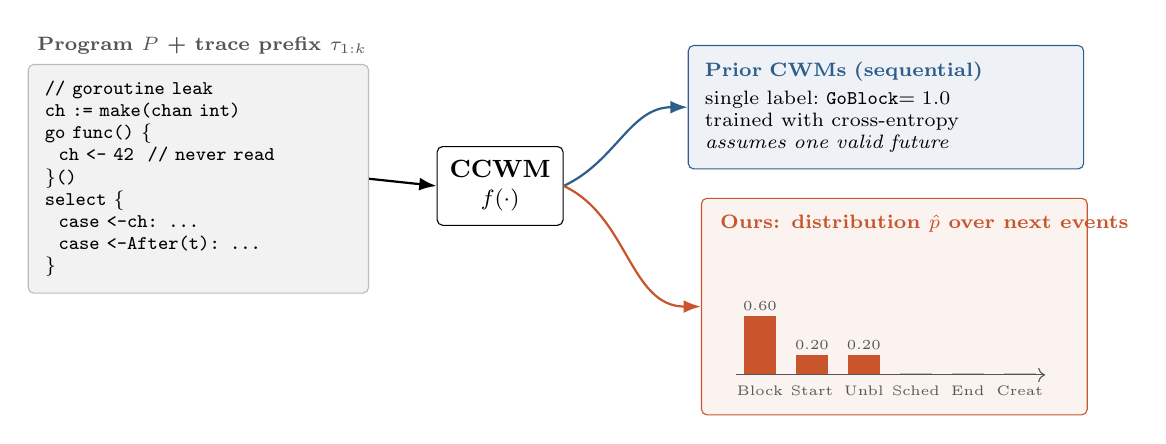
\begin{tikzpicture}[font=\sffamily]

\node[anchor=north west,align=left,font=\ttfamily\scriptsize,
      fill=panelgray,draw=panelborder,rounded corners=2pt,
      inner sep=6pt,text width=3.9cm] (prog) at (0,0)
{// goroutine leak\\
ch := make(chan int)\\
go func() \{\\
\ \ ch <- 42 \ // never read\\
\}()\\
select \{\\
\ \ case <-ch: ...\\
\ \ case <-After(t): ...\\
\}};
\node[anchor=south west,font=\bfseries\scriptsize,labelone]
      at (prog.north west) {Program $P$ + trace prefix $\tau_{1:k}$};

\node[draw,fill=white,rounded corners=2pt,minimum height=1.0cm,
      minimum width=1.6cm,align=center,font=\small\bfseries]
      (model) at (6.0,-1.55) {CCWM\\[-1pt]\footnotesize $f(\cdot)$};
\draw[-{Latex[length=2.2mm]},thick] (prog.east) -- (model.west);

\node[draw=cwmblue,fill=cwmblue!8,rounded corners=2pt,
      inner sep=6pt,align=left,font=\scriptsize,text width=4.6cm]
      (cwm) at (10.9,-0.55)
{\textbf{\color{cwmblue}Prior CWMs (sequential)}\\[2pt]
single label:\ \texttt{GoBlock}$=1.0$\\
trained with cross-entropy\\
\emph{assumes one valid future}};

\node[draw=oursorange,fill=oursorange!7,rounded corners=2pt,
      minimum width=4.9cm,minimum height=2.75cm,anchor=north west]
      (ourspanel) at (8.55,-1.7) {};
\node[anchor=north west,font=\scriptsize\bfseries,oursorange,align=left]
      at ($(ourspanel.north west)+(0.12,-0.1)$)
      {Ours: distribution $\hat p$ over next events};

\begin{scope}[shift={($(ourspanel.north west)+(0.55,-2.25)$)}]
  \def\gap{0.66}\def\bw{0.40}\def\h{1.25}
  \foreach \i/\p/\lab in {0/0.60/Block,1/0.20/Start,2/0.20/Unbl,3/0.00/Sched,4/0.00/End,5/0.00/Creat}{
    \pgfmathsetmacro\bh{\p*\h}
    \ifdim\bh pt>0.01pt
      \fill[barfill] ({\i*\gap},0) rectangle ({\i*\gap+\bw},{\bh});
      \node[font=\tiny,labelone] at ({\i*\gap+\bw/2},{\bh+0.13}) {\p};
    \else
      \draw[panelborder] ({\i*\gap},0) rectangle ({\i*\gap+\bw},0.02);
    \fi
    \node[font=\tiny,labelone,anchor=north] at ({\i*\gap+\bw/2},-0.02) {\lab};
  }
  \draw[->,labelone] (-0.1,0) -- ({5*\gap+\bw+0.12},0);
\end{scope}

\draw[-{Latex[length=2.2mm]},thick,cwmblue] (model.east) to[out=25,in=180] (cwm.west);
\draw[-{Latex[length=2.2mm]},thick,oursorange] (model.east) to[out=-25,in=180]
      ($(ourspanel.west)+(0,0.0)$);

\end{tikzpicture}
\end{document}
